\chapter{ตรีโกณมิติเบื้องต้น}
ยินดีต้อนรับเข้าสู่บทเรียนเรื่องตรีโกณมิติ เอกสารเล่มนี้ประกอบไปด้วยหัวข้อและสรุปใจความสำคัญต่างๆ

\begin{agreementbox}
	สัญลักษณ์ต่าง ๆ ตลอดเนื้อหาของเอกสารฉบับนี้ มีความหมายดังนี้
	\begin{enumerate}
		\item สัญลักษณ์ $\times$ และ $\cdot$ หมายถึง เครื่องหมายคูณ
		\item สัญลักษณ์ $\angle A$ หรือ $\hat{A}$ หมายถึง ขนาดของมุม $A$
		\item สัญลักษณ์ $\triangle ABC$ หมายถึง สามเหลี่ยม $ABC$ และ $[\triangle ABC]$ หมายถึง พื้นที่ของ $\triangle ABC$
		\item สัญลักษณ์ $\square ABCD$ หมายถึง สี่เหลี่ยม $ABCD$ และ $[\square ABCD]$ หมายถึง พื้นที่ของ $\square ABCD$
		\item ให้ $\ell_1$ และ $\ell_2$ แทนเส้นตรงสองเส้น สัญลักษณ์ $\ell_1 // \ell_2$ หมายถึง เส้นตรง $\ell_1$ และ $\ell_2$ ขนานกัน
	\end{enumerate} 
\end{agreementbox}

\section{อัตราส่วนตรีโกณมิติ}
\subsection{อัตราส่วนตรีโกณมิติพื้นฐานที่ควรรู้}

\begin{definitionbox}[ฟังก์ชันตรีโกณมิติ] \label{defition1}
	บทนิยามของฟังก์ชันตรีโกณมิติที่คำนวณจากรูปสามเหลี่ยมมุมฉาก
\end{definitionbox}
จากนิยาม \ref{defition1} 

\subsection{ค่าฟังก์ชันตรีโกณมิติของมุมพื้นฐาน}
ตารางต่อไปนี้แสดงค่าฟังก์ชันตรีโกณมิติของมุมพื้นฐานที่ใช้บ่อย ในหน่วยองศา

\begin{table}[h]
	\centering
	% ปรับระยะห่างระหว่างคอลัมน์ให้กว้างขึ้นเล็กน้อย
	\setlength{\tabcolsep}{8pt} 
	
	% ใช้ C แทน c เพื่อเปิดใช้งาน cellspace (เพิ่มช่องว่างบน-ล่าง)
	\begin{tabular}{| Sc | Sc | Sc | Sc | Sc | Sc | Sc | Sc | Sc |}
		\hline
		$\theta\,\text{(องศา)}$ 
		& $0^\circ$ 
		& $30^\circ$ 
		& $45^\circ$ 
		& $60^\circ$ 
		& $90^\circ$ 
		& $180^\circ$
		& $270^\circ$
		& $360^\circ$ \\
		\hline
		
		$\sin(\theta)$ 
		& $0$ 
		& $\dfrac{1}{2}$ 
		& $\dfrac{\sqrt{2}}{2}$ 
		& $\dfrac{\sqrt{3}}{2}$ 
		& $1$ 
		& $0$ 
		& $-1$ 
		& $0$ \\ 
		\hline
		
		$\cos(\theta)$ 
		& $1$ 
		& $\dfrac{\sqrt{3}}{2}$ 
		& $\dfrac{\sqrt{2}}{2}$ 
		& $\dfrac{1}{2}$ 
		& $0$ 
		& $-1$ 
		& $0$ 
		& $1$ \\
		\hline
		
		$\tan(\theta)$ 
		& $0$ 
		& $\dfrac{1}{\sqrt{3}}$ 
		& $1$ 
		& $\sqrt{3}$ 
		& \text{ไม่กำหนดค่า}
		& $0$ 
		& \text{ไม่กำหนดค่า} 
		& $0$ \\
		\hline
	\end{tabular}
	\caption{ค่าฟังก์ชันตรีโกณมิติของมุมพื้นฐานในหน่วยองศา}
	\label{table1.1}
\end{table}

\begin{observationbox}
	เนื่องจาก $\sin(A)=\dfrac{a}{c},\,\,\cos(A)=\dfrac{b}{c}$ และ $\tan(A)=\dfrac{a}{b}$\\
	\vspace{0.5cm}\\
	จะเห็นได้ว่า $\tan(A)=\dfrac{\sin(A)}{\cos(A)}$ และ $\cot(A)=\dfrac{\cos(A)}{\sin(A)}$    
\end{observationbox}

\begin{examplebox} \label{examplebox1}
	จงหาค่าของ $\arcsin 30^\circ + \arccos 60^\circ +\arctan 60^\circ$
\end{examplebox}
\begin{examplebox} \label{examplebox2}
	จงหาค่าของ $\sin 30^\circ + \cos 60^\circ$
\end{examplebox}
\begin{examplebox} \label{examplebox3}
	จงหาค่าของ $\sin 30^\circ + \cos 60^\circ$
\end{examplebox}
จากตัวอย่าง \ref{examplebox1} เราได้ว่า\\
จากตัวอย่าง \ref{examplebox2} เราได้ว่า\\
จากตัวอย่าง \ref{examplebox3} เราได้ว่า

\begin{remarkbox} \label{remarkbox1}
	ตัวอย่างการทดสอบระบบกล่องข้อควรรู้แบบกรอบเส้นประสีพาสเทล
\end{remarkbox}

\subsection{องศาและเรเดียน}
\begin{conceptbox}
	\begin{itemize}
		\item[*] เปลี่ยน \textbf{เรเดียน} เป็น \textbf{องศา} แทน $\pi$ ด้วย $180^{\circ}$ 
		\item[*] เปลี่ยน \textbf{องศา} เป็น \textbf{เรเดียน} คูณด้วย $\dfrac{\pi}{180}$
	\end{itemize}   
\end{conceptbox}

\begin{examplebox}[NETSAT คณิตศาสตร์ กุมภาพันธ์ 2567]  
	$72^{\circ}$ เท่ากับกี่เรเดียน
	\begin{enumerate}
		\item $\dfrac{2\pi}{3}$
		\item $\dfrac{2\pi}{5}$
		\item $\dfrac{3\pi}{4}$
		\item $\dfrac{3\pi}{5}$
	\end{enumerate}
\end{examplebox}

\begin{theorembox}[กฏของไซน์]
	กำหนดให้ $\triangle ABC$ ถูกล้อมรอบด้วยวงกลมรัศมี $R$ แต่มีความยาวแต่ละด้านซึ่งแสดงดังรูปที่~\ref{Figure26} เราจะได้ความสัมพันธ์ว่า
	\[\frac{a}{\sin(A)}=\frac{b}{\sin(B)}=\frac{c}{\sin(C)}=2R\]
\end{theorembox}
\begin{figure}[H]	 
	\centering
	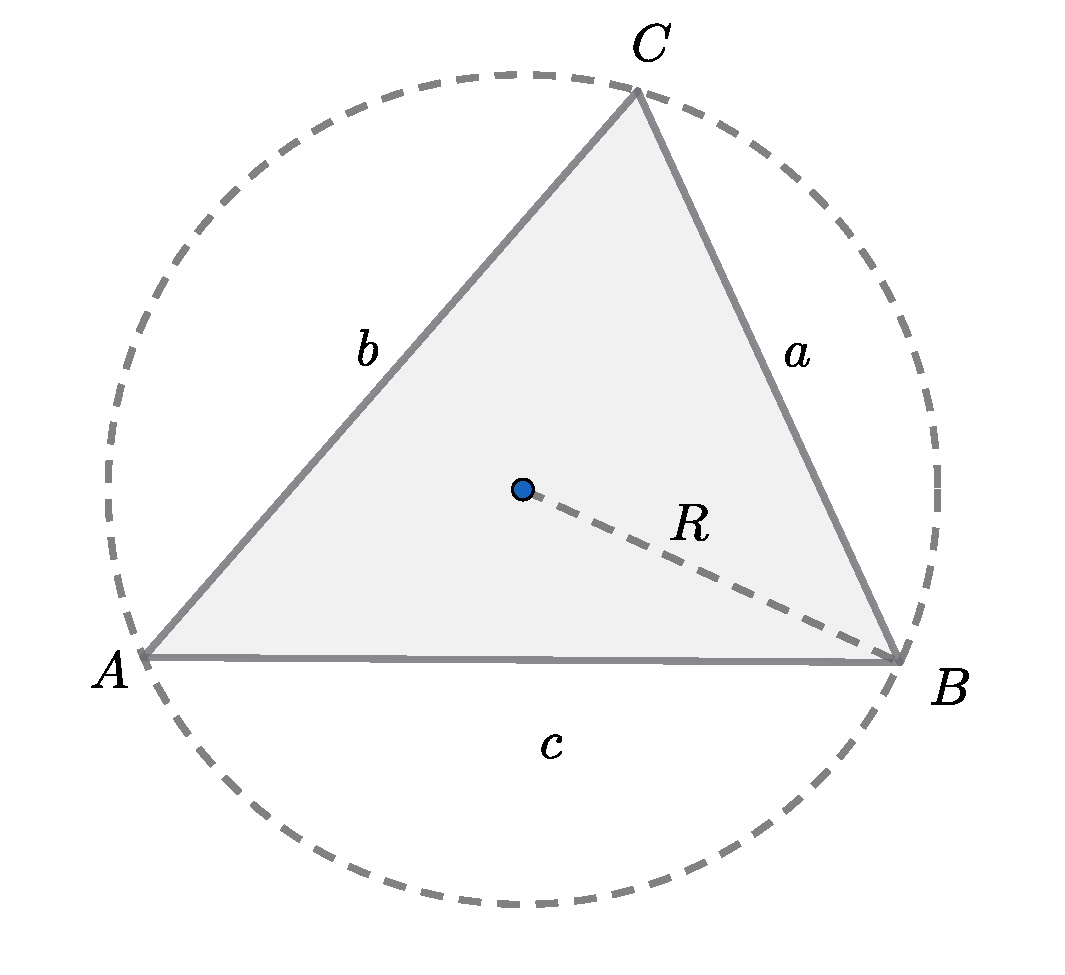
\includegraphics[scale=0.4]{26}
	\caption{}
	\label{Figure26}
\end{figure} 